\section{Data Sources and Data Preparation}

\begin{figure}
\centering
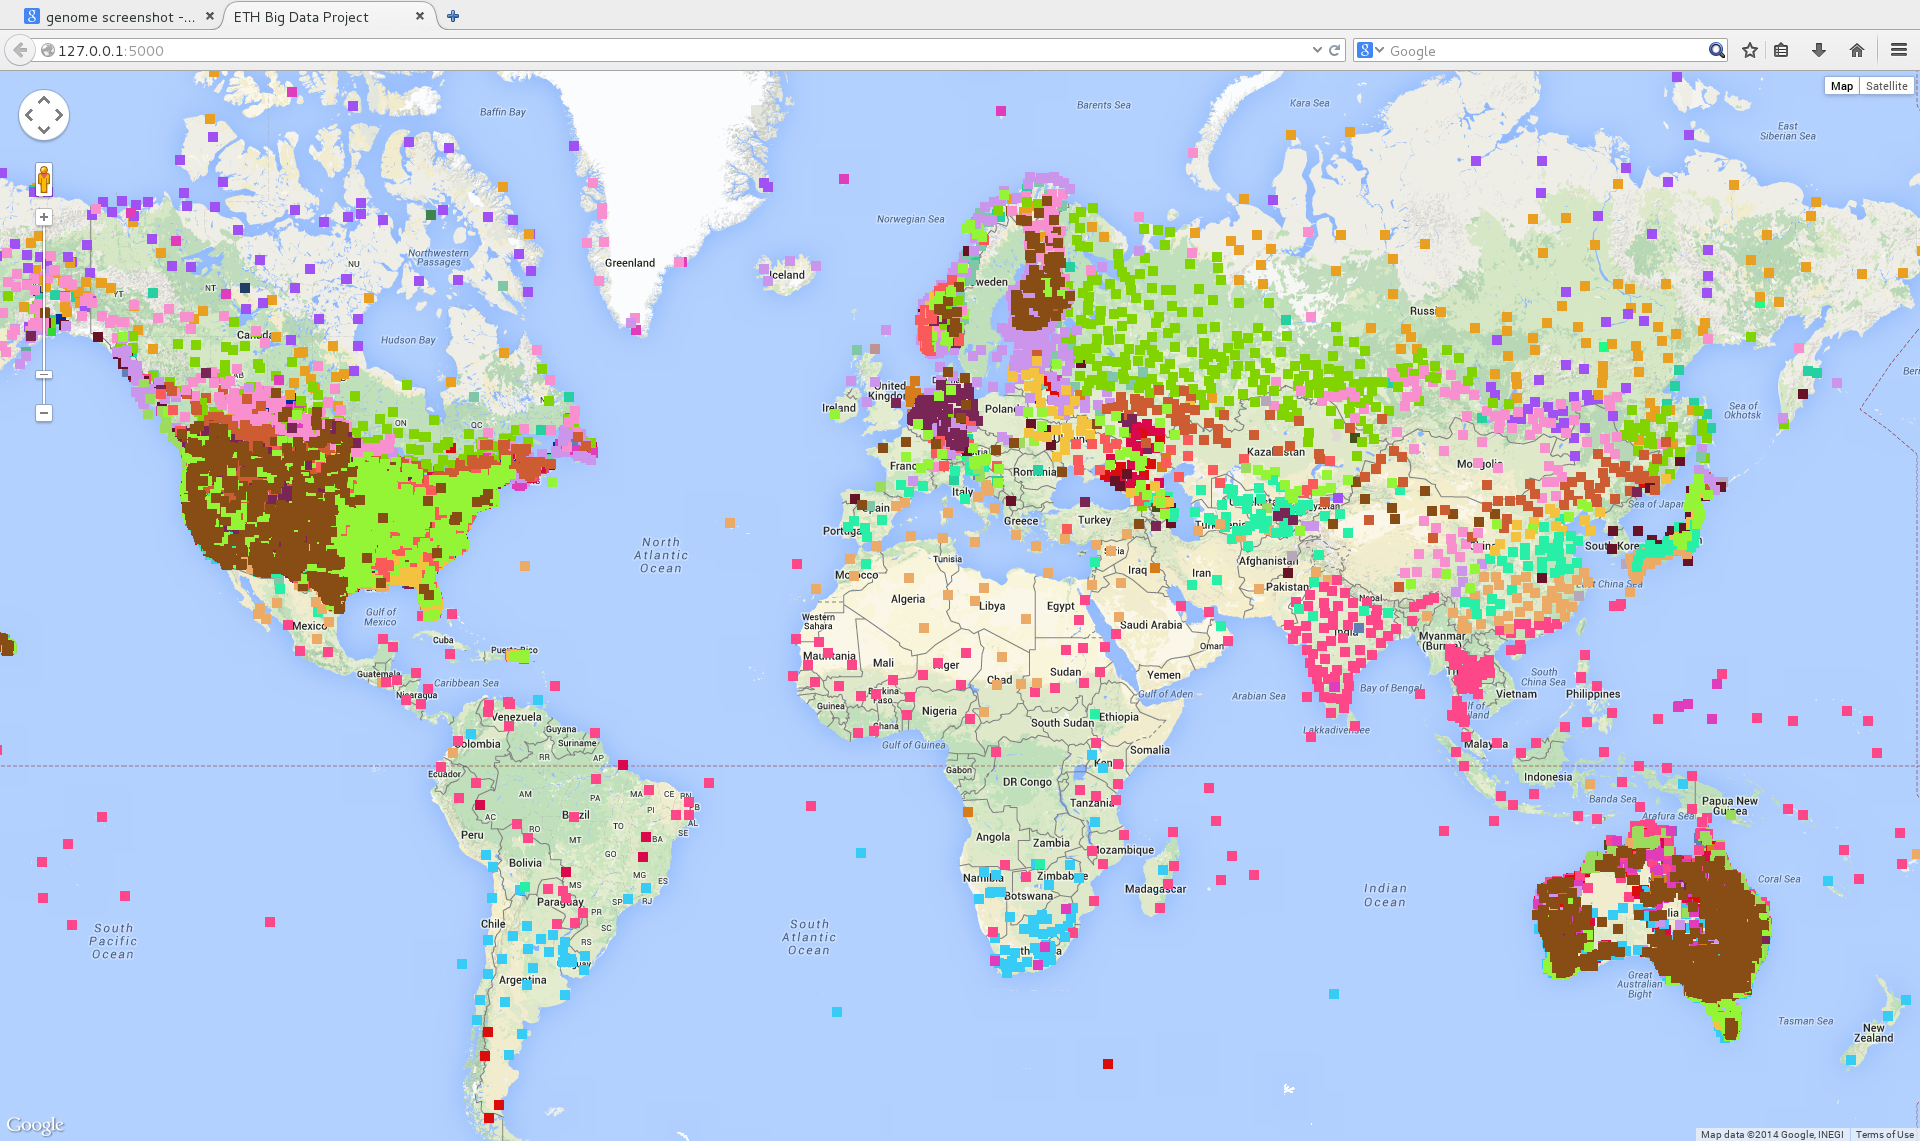
\includegraphics[width=.85\linewidth]{./figure/Full_view.png}
	\caption{Visualization of climate pattern clustering with our system.}
	\label{fig:FullView}
\end{figure}

\subsection{Introduction}
GHCN-D is a dataset that contains daily weather observations over global land areas.
Like its monthly counterpart, GHCN-Daily is a composite of climate records from
numerous sources that were merged together and subjected to a common suite of quality
assurance reviews. The archive includes the following meteorological elements: daily maximum temperature, daily minimum temperature, temperature at the time of observation, precipitation (i.e., rain, melted snow), snowfall, snow depth, other elements where available.

We use an alternate form of the GHCN Daily dataset. The period of record station files are parsed into
yearly files that contain all available GHCN Daily station data for that year
plus a time of observation field (where available--primarily for U.S. Cooperative
Observers).  The obsertation times for U.S. Cooperative Observer data
come from the station histories archived in NCDC's Multinetwork Metadata System (MMS).

The yearly files are formatted so that every observation
%(i.e.,station/year/month/day/element/observation time)
 is represented by a single row
with the following fields:
station identifier (GHCN Daily Identification Number)
, date (yyyymmdd; where yyyy=year; mm=month; and, dd=day), observation type (see ftp://ftp.ncdc.noaa.gov/pub/\\data/ghcn/daily/readme.txt for definitions), observation value (see ftp://ftp.ncdc.noaa.gov/pub/\\data/ghcn/daily/readme.txt for units), observation time (if available, as hhmm where hh=hour and mm=minutes in local time). One sample data record goes as the following: 

US1FLSL0019,20090101,PRCP,0,,,N.
% \subsection{Data Extraction}
%
% For milestone $2$, we took the year file of 2013, extracted the five key elements, and collected by station identifiers.


%{\color{red} Menne, M.J., I. Durre, R.S. Vose, B.E. Gleason, and T.G. Houston, 2012:  An overview
%of the Global Historical Climatology Network-Daily Database.  Journal of Atmospheric
%and Oceanic Technology, 29, 897-910, doi:10.1175/JTECH-D-11-00103.1.}
